Figure~\ref{fig:unfolded_pt} presents the unfolded underlying event observable, 
$\langle \Sigma E_{T}/\delta\eta\delta\phi \rangle$, as a function of the leading jet transverse momentum for both inclusive jet and dijet event selections. The results are compared to generator-level predictions from \pythia and \herwig.
UE decreases with increasing jet $p_{T}$ showing an anti-correlation between the hard scattering scale and soft particle production at RHIC energies. 
This is the opposite of the behavior seen in inclusive jet events at the LHC, where higher-$Q^{2}$ scatterings are more likely to have ISR and FSR, and a more central overlap of the colliding nucleons with more MPI, all resulting in increased UE activity. 
Instead, the transverse region average energy density decreases with increasing jet $p_{T}$ indicating that the interplay between soft and hard processes at RHIC energies is more detailed than just radiation effects. 

\begin{figure}
    \centering
    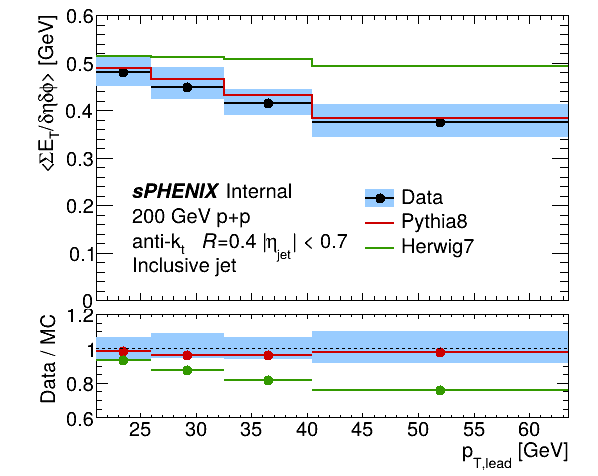
\includegraphics[width=0.7\linewidth]{ueinpp/Figures/h_result_inclusive.png}
    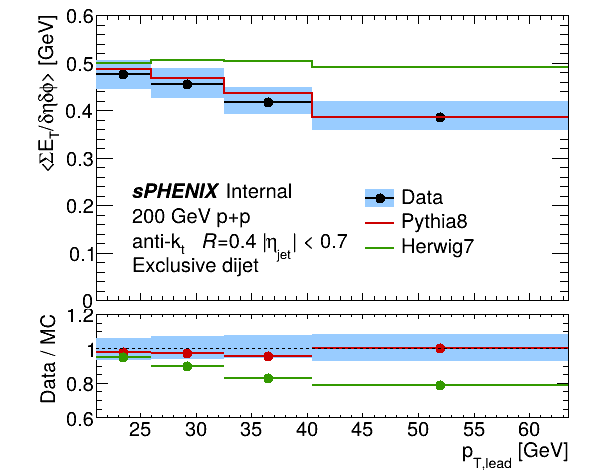
\includegraphics[width=0.7\linewidth]{ueinpp/Figures/h_result_dijet.png}
    \caption{Transverse region average energy density, $\langle \Sigma E_{T}/\delta\eta\delta\phi \rangle$, as a function of leading jet $p_{T}$ for inclusive jet (left) and dijet (right) event selections. Data (black points) are shown with statistical uncertainties (bars) and systematic uncertainties (blue bands). The results are compared to generator-level predictions from \pythia (red line) and \herwig (green line).}
    \label{fig:unfolded_pt}
\end{figure}

Comparing to the data, \pythia reproduces both the overall magnitude and trend with jet $p_{T}$ seen in data. In the low jet $p_{T}$ range of the measurement, \herwig agrees fairly well with the data but does not reproduce the overall anti-correlation between the UE and jet $p_{T}$ seen in data. Both \pythia and \herwig incorporate MPI with impact-parameter dependence and include ISR and FSR. However, in \pythia, MPI are interleaved with the parton shower evolution allowing for tunable competition between the soft and hard processes. While in \herwig, MPI and parton showers are included in the model separately. Therefore, the underlying event activity is modeled to be fairly independent of the hard scattering scale. The measurement of the UE as a function of jet $p_T$ here helps discriminate between these two approaches to collision event modeling and better constrains the description of soft--hard interplay in p+p collisions at RHIC energies.

For both the inclusive jet and exclusive dijet selections, the $\langle \Sigma E_{T}/\delta\eta\delta\phi\rangle$ decreases with increasing leading jet $p_{T}$.
While the systematic uncertainty on the measurements are large ($\sim \pm 8\%$), the uncertainties are highly correlated between different leading jet $p_{T}$ bins and thus the trend of the measurement is more robust than the overall normalization.
The overall uncertainty is dominated by scale uncertainties from the hadronic response and noise uncertainties, which can be factored out when making comparisons between different jet $p_{T}$ bins or different event selections.
Therefore, the shape of the distribution and its dependence on the hard scale are more precisely constrained than the absolute scale, and the anti-correlation seen in Figure~\ref{fig:unfolded_pt} is significant within uncorrelated uncertainties. 

\begin{figure} 
    \centering
    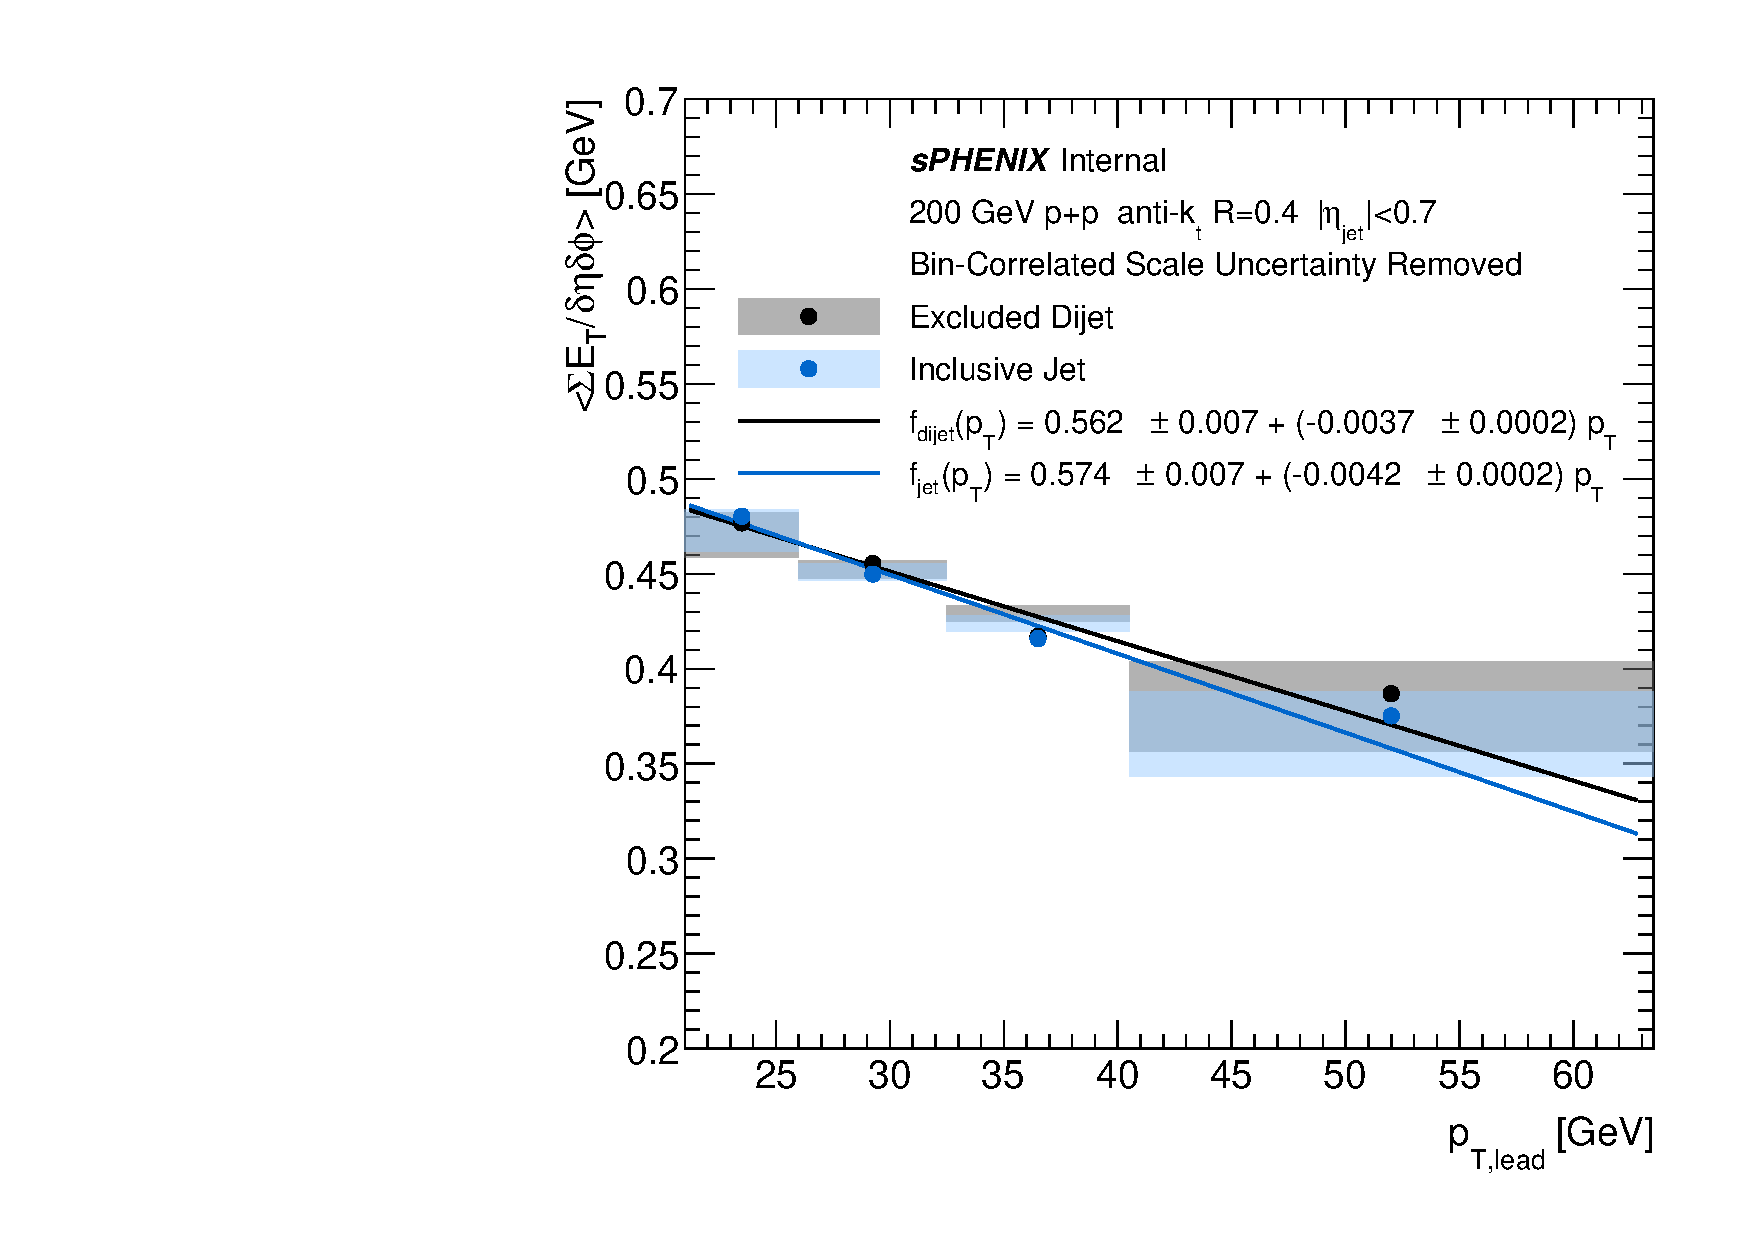
\includegraphics[width=0.5\linewidth]{figures/chapter5/h_jet_pt_bin_unc_figure.pdf}
    \caption{Transverse region average energy density, $\langle \Sigma E_{T}/\delta\eta\delta\phi \rangle$, as a function of leading jet $p_{T}$ for inclusive jet (blue points) and dijet (black points) event selections. Data are shown with statistical uncertainties (bars) and shape-only systematic uncertainties (bands). Bin-correlated scale uncertainties have been removed to highlight trend as a function of leading jet $p_{T}$. Functional linear fits (lines) are shown for inclusive jet and dijet results.}
    \label{fig:bin_by_bin_comp}
\end{figure}

Figure~\ref{fig:bin_by_bin_comp} shows the trend of $\langle \Sigma E_{T}/\delta\eta\delta\phi\rangle$ as a function of jet $p_{T}$ where the overall scale uncertainty is removed by fitting the trend to a linear fit and extracting the slope for each variation, providing an overall uncertainty on the bin-by-bin shape of the distribution. 

\begin{figure}
    \centering
    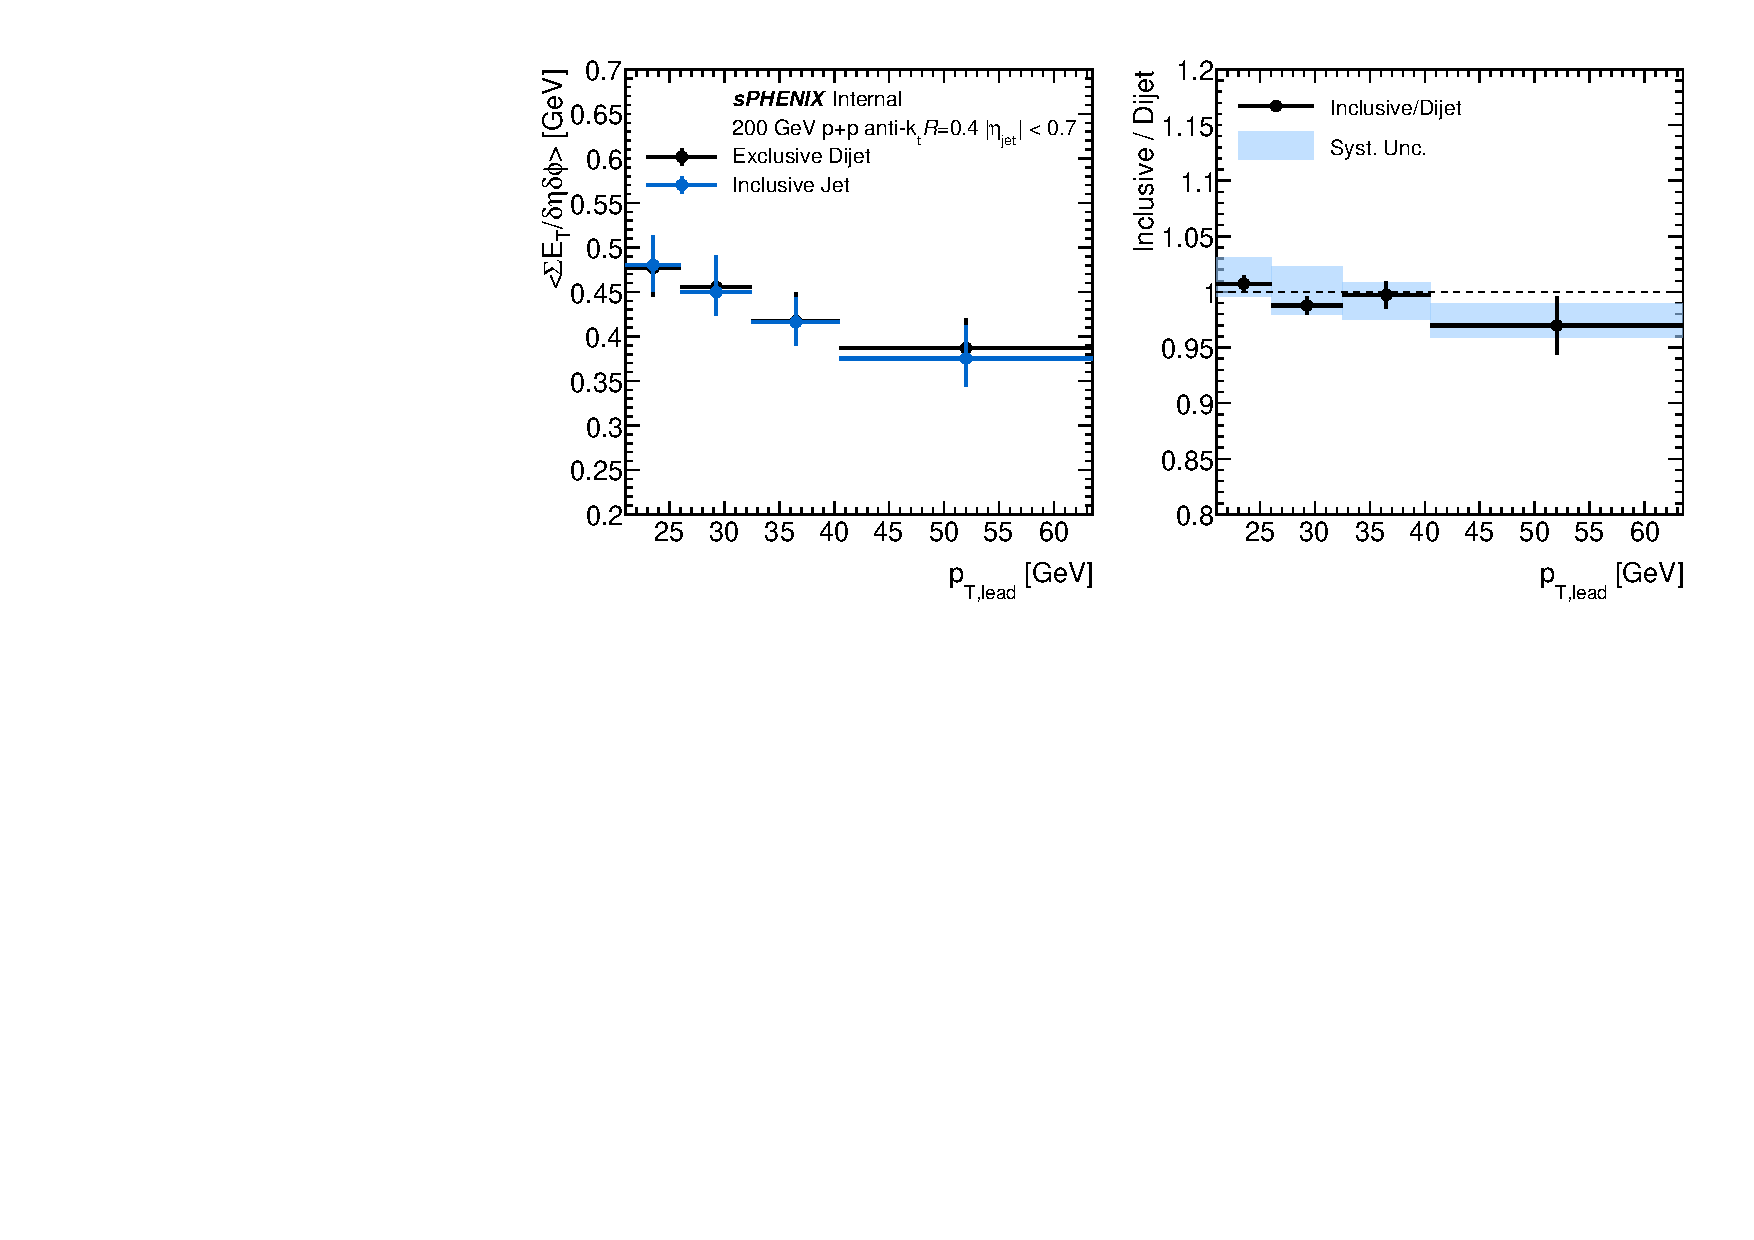
\includegraphics[width=\linewidth]{figures/chapter5/h_compare_efrac_over_dijet_shape_only_unc_figure.pdf}
    \caption{Left: Transverse region average energy density, $\langle \Sigma E_{T}/\delta\eta\delta\phi \rangle$, as a function of leading jet $p_{T}$ for inclusive jet (blue points) and dijet (black points) event selections. Data are shown with statistical and systematic uncertainties (bars). Right: Ratio of inclusive jet to dijet result (black points) with uncorrected systematic uncertainties (blue band).}
    \label{fig:inclusive_dijet_comp}
\end{figure}

Additionally, the inclusive jet and exclusive dijet measurements are in agreement within their uncorrelated uncertainties, indicating that the UE measurement is not significantly sensitive to requiring a dijet event selections at RHIC energies.
Figure~\ref{fig:inclusive_dijet_comp} directly compares the results from the inclusive jet measurement and the dijet measurement; these results show fairly good agreement with uncorrelated systematic and statistical uncertainties. 
This very similar trend between the inclusive and dijet results greatly contrasts with the ATLAS inclusive and dijet results which show very different trends. 

A comparison of the sPHENIX inclusive jet and dijet results to the ATLAS results~\cite{ATLAS:2014underlying_event_jets_7tev} for inclusive jet and dijet result as a function of parton x is shown in Figure~\ref{fig:atlas_comp}. Here, the sPHENIX results are lower than the ATLAS results for both event selections across the full parton x range.
Note here a proxy for parton x based on the leading jet $p_{T}$ is used: 
\begin{equation}
    x = \frac{2p_{T}}{\sqrt{s}}
\end{equation}
A comparison of the ATLAS results~\cite{ATLAS:2014underlying_event_jets_7tev} to the STAR results~\cite{STAR:2024underlying_event_pp_200gev} and sPHENIX results determined by using the $<p_{T}>$ information also measured by STAR are shown in Figure~\ref{fig:star_atlas_comp}. Here, the RHIC results are lower than the ATLAS results for both event selections across the full parton x range. Fairly good agreement between the sPHENIX and STAR results are observed across the full parton x range. The sPHENIX $dN_{ch}/d\eta d\phi$ is approximately calculated as the following:
\begin{equation}
    \langle dN_{ch}/d\eta d\phi \rangle = \frac{2}{3}\frac{\langle dE_{T}/d\eta d\phi \rangle}{\langle p_{T} \rangle}
\end{equation}
where the factor of 2/3 comes from the fraction of charged particles and the $\langle p_{T} \rangle$ value for the UE particles as a function of leading jet $p_{T}$ was also pulled from the STAR measurement~\cite{STAR:2024underlying_event_pp_200gev}.

\begin{figure}
    \centering
    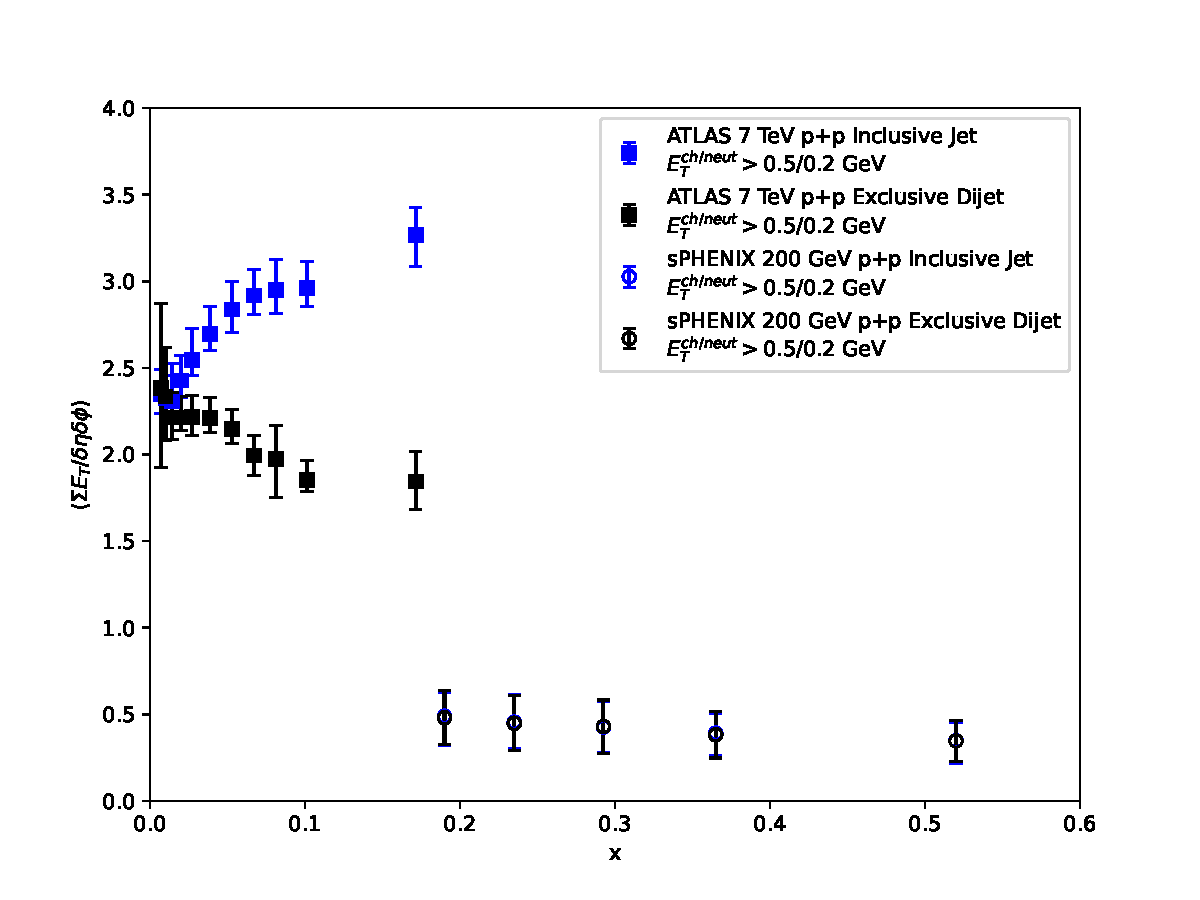
\includegraphics[width=0.8\linewidth]{figures/chapter5/et_dens_comp_sphenix_atlas.pdf}
    \caption{Comparison of transverse region average energy density, $\langle \Sigma E_{T}/\delta\eta\delta\phi \rangle$, as a function of parton $x$ for inclusive jet (blue) and dijet (black) event selections. sPHENIX data from 200 GeV p+p collisions (open circles) are compared ATLAS results from 7 TeV p+p collisions (filled squares). Data are shown with statistical uncertainties and systematic uncertainties (bars).}
    \label{fig:atlas_comp}
\end{figure}
\begin{figure}
    \centering
    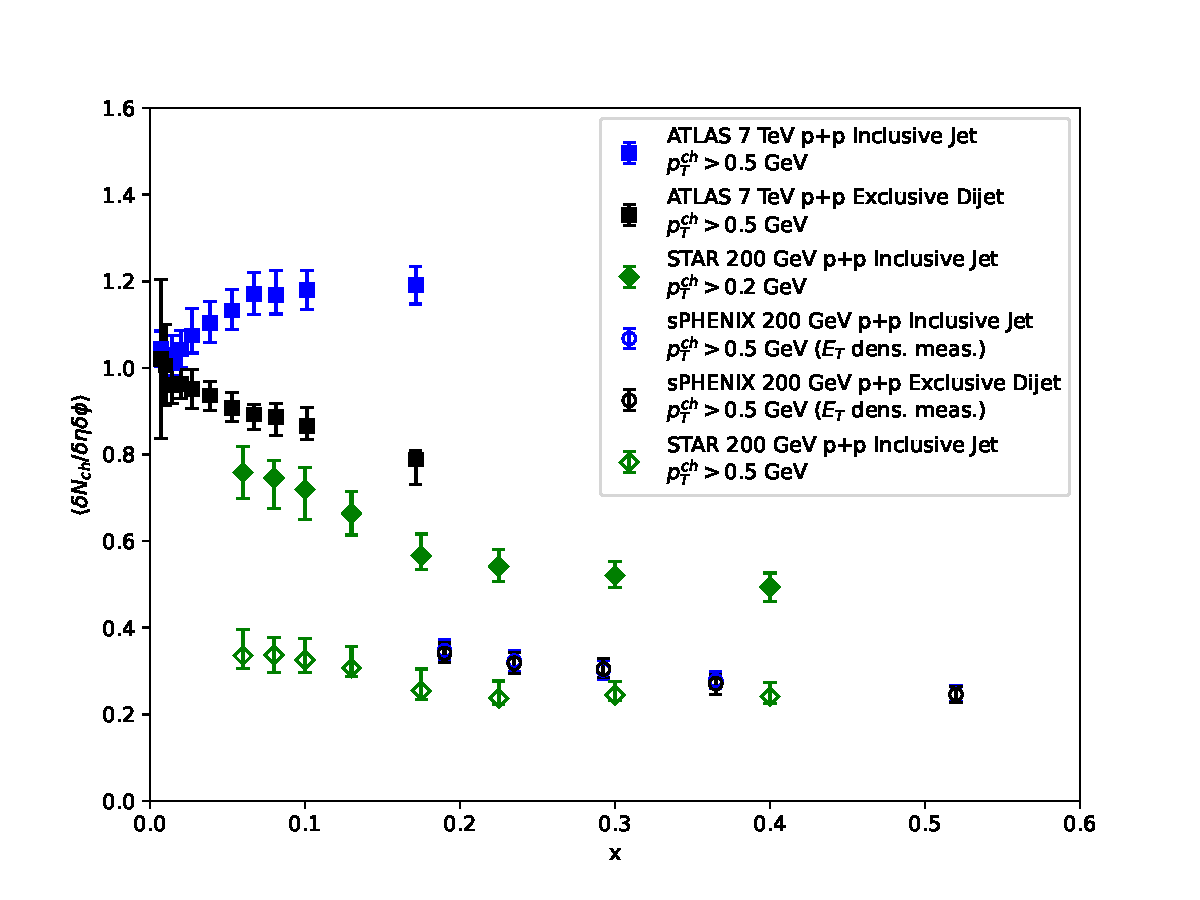
\includegraphics[width=0.8\linewidth]{figures/chapter5/nch_dens_comp_sphenix_star_atlas.pdf}
    \caption{Comparison of transverse region average charged particle multiplicity, $\langle \delta N_{ch}/\delta\eta\delta\phi \rangle$, as a function of parton $x$. sPHENIX inclusive jet (blue) and exclusive dijet (black) data from 200 GeV p+p collisions (open circles) are compared ATLAS results from 7 TeV p+p collisions (filled squares) and STAR inclusive jet results (green) from 200 GeV p+p collisions with $p^{ch}_{T}$ threshold of 0.2 GeV (filled diamond) and 0.5 GeV (open diamond). Data are shown with statistical uncertainties and systematic uncertainties (bars).}
    \label{fig:star_atlas_comp}
\end{figure}